\section{Theorie}
\label{sec:Theorie}
Laser steht für „Light Amplification by Stimulated Emission of Radiation“.
Er ist in der Forschung, speziell in der Spektroskopie, von großer Bedeutung, da er eine ideale Lichtquelle darstellt.
Das Licht eines idealen Lasers ist kohärent, monochromatisch, hat eine hohe Intensität und hält diese stabil.
Im Folgenden soll am Beispiel des Diodenlasers erläutert werden, wie eine solche Lichtquelle realisiert werden kann und 
wie er für die Spektroskopie der Hyperfeinstrukturaufspaltung von Rubidium genutzt werden kann.
\subsection{Funktionsweise eines Lasers}
Grundlegend besteht ein Laser aus drei Komponenten: einem aktiven Medium, einer Energiepumpe und einem Resonator.
Die Energiepumpe pumpt Energie in das System, indem Elektronen im aktiven Medium angeregt werden (z.B. über eine Blitzlampe, Gasentladung,einem weiteren Laser oder wie in dem Fall über einen Strom von Ladungen).
Das Ziel der Energiepumpe ist es, eine Besetzungsinversion zu erzeugen. Das heißt, wie in Abbildung \ref{fig:inv} zu sehen, einen Zustand hoher Energie mit einer größeren Anzahl Elektronen zu besetzen 
als die energetisch darunter liegenden Zustände.
\begin{figure}[H]
    \centering
    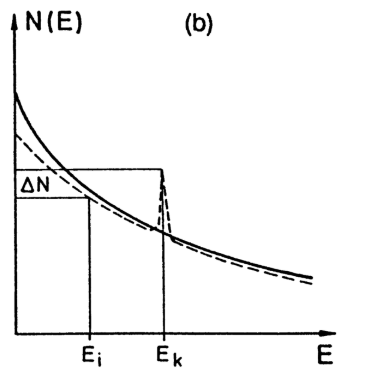
\includegraphics[scale=0.9]{pictures/Inv.png}
    \caption{Besetzungsverteilung eines aktiven Mediums\cite{Demtröder}.}
    \label{fig:inv}
\end{figure}
\noindent Die Elektronen regen sich durch verschiedene Emissionsprozesse unter Aussendung eines Photons fester Energie ab.
Die Photonen werden dann im Resonator reflektiert und so wieder durch das aktive Medium hindurch geschickt,
wo sie durch stimulierte Emission weitere Photonen erzeugen. Dadurch wird der Laser zu einem selbstschwingenden Oszillator.
Diese Photonen sind dann kohärent. Ein Resonatorspiegel ist teildurchlässig, wodurch sich nach hochfahren des Lasers ein Maximum einstellt. Danach wird durch den teildurchlässigen
Spiegel eine konstante Lichtintensität abgegeben. Je nach Resonatorkonfiguration speichert der Laser das Licht in festen Moden.
\subsection{Emission und Absorption im Aktiven Medium}
Zunächst sollten die wichtigsten Prozesse im aktiven Medium, anhand eines Zwei-Niveau-Systems diskutiert werden. 
Wie in Abbildung \ref{fig:Prozesse} zu sehen, gibt es drei zentrale Prozesse. Liegt ein System in einem angeregten Zustand vor, heißt das, dass ein Elektron auf dem Zustand höherer Energie vorliegt.
Es ist grundsätzlich energetisch günstiger für das Elektron in einem tieferen Zustand vorzuliegen. Tritt dieser Übergang ohne äußere Einflüsse auf, so wird ein Photon mit der entsprechenden Energiedifferenz zwischen den beiden Niveaus ausgesendet. Dies wird spontane Emission genannt.
Bewegt sich nun ein Photon mit genau der Energiedifferenz zweier Zustände eines Atoms auf dieses zu, kann es zu 2 Prozessen kommen.
Wenn das Elektron im niedrigeren Zustand vorliegt, kann das Photon absorbiert werden (Absorption) und 
das Elektron in den höheren Zustand übergehen. Liegt das Elektron im höheren Zustand vor, kann das Photon eine stimulierte Emission auslösen, bei der 
das Elektron in den niedrigeren Zustand übergeht und ein weiteres kohärente Photon aussendet. Das Photon hat dann gleiche Wellenlänge, Polarisation und Ausbreitungsrichtung wie das ursprüngliche Photon.
\begin{figure}[H]
    \centering
    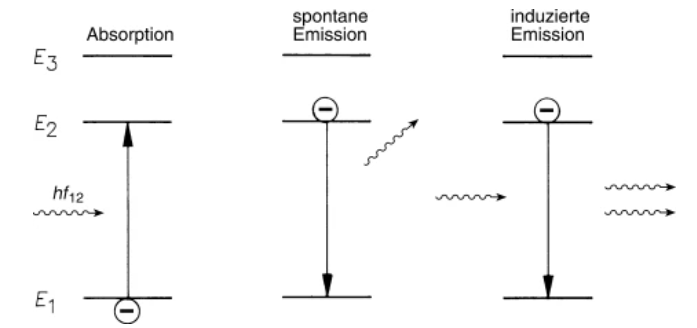
\includegraphics[scale=0.9]{pictures/Prozesse.png}
    \caption{Übergänge zwischen Energieniveaus\cite{Eichler20152}.}
    \label{fig:Prozesse}
\end{figure}
Damit die für den Laser wichtige Besetzungsinversion erzeugt wird, muss der Laser mindestens ein 3-Niveau-System besitzen.
Denn in einem 2-Niveau System würden sich stimulierte Emission und Absorption gegenseitig aufheben, da die Wahrscheinlichkeit für beide Prozesse gleich ist.
In einem Halbleiterlaser mit einer kontinuierlichen Bandstruktur ist dies automatisch gegeben.
\subsection{Halbleiter}
In Festkörpern mit einem periodischen Gitter kann die Besetzung der Elektronen über eine Bandstruktur beschrieben werden.
Nach dem Pauli-Prinzip können zwei Elektronen in einem System nicht die gleichen Energieniveaus besetzen. Daher spalten sich 
die Energieniveaus der einzelnen Atome in ein Band auf. Genauer sind die Energiebänder die Überlagerungen der Energieniveaus aller Atome im 
reziproken Raum. Dementsprechend können Elektronen mit einer bestimmten Energie im Festkörper nur vorliegen, wenn es Zustände in einem Band mit dieser 
Energie gibt. Energieintervalle ohne Zustand werden Bandlücken genannt, da dort keine Elektronen existieren können.

\noindent Festkörper können anhand ihrer Bandstruktur in 3 Kategorien unterteilt werden: Metalle, Halbleiter und Isolatoren.
Die Bandstruktur dieser Festkörper ist in Abbildung \ref{fig:Band} dargestellt.
\begin{figure}[H]
    \centering
    \includegraphics[scale=0.8]{pictures/Bänder.png}
    \caption{Bandstruktur von Metallen, Halbleitern und Isolatoren \cite{demtröder}.}
    \label{fig:Band}
\end{figure}
\noindent Dabei bezeichnet $E_\text{F}$ die Fermi-Energie, welche angibt bis zu welcher Energie bei $T=\qty{0}{\kelvin}$ die Zustände besetzt sind.
Bei Isolatoren liegt diese Energie zwischen 2 Bändern, also in einer Bandlücke. Das Band unterhalb der Fermi-Energie wird Valenzband genannt, 
da dieses bei $T=\qty{0}{\kelvin}$ vollständig besetzt ist. Das Band oberhalb der Fermi-Energie wird Leitungsband genannt, da dieses bei $T=\qty{0}{\kelvin}$ leer ist und 
Elektronen in diesem Band frei beweglich sind. Bei Metallen liegt die Fermi-Energie im Leitungsband, weshalb diese bei $T=\qty{0}{\kelvin}$ leitfähig sind.
Halbleiter haben eine analoge Bandstruktur zu Isolatoren, jedoch ist die Bandlücke kleiner. Sie beträgt bei Halbleitern bis zu $\qty{3}{\eV}$, bei Isolatoren 
ist sie größer. Daher können in Halbleitern durch thermische Anregung, bei Raumtemperatur etwa $\qty{26}{\milli\eV}$, Elektronen in das Leitungsband gelangen. 
Allerdings ist die Ladungsträgerdichte in Eigenleitung noch sehr gering. In diesem Versuch wird ein Aluminium-Gallium-Arsenid-Halbleiter(AlGaAs) verwendet. Dieser kann als "Light emitting Diode" (LED)
durch Rekombination von Elektronen und Löchern Licht emittieren. Die Bandlücke liegt im infrarotem Wellenlängenbereich von $\qty{780}{\nano\meter}$.
Entscheidend für die Funktionsweise eines Diodenlasers ist nun auch die Biegung der Bänder im p-n-Übergang. Bei angelegter Spannung können 
Driftströme das E-Feld der Verarmungszone überwinden und Ladungen sammeln sich bereit zum Rekombinieren in der Verarmungszone.
Dies ist schematisch in Abbildung \ref{fig:PN} dargestellt. 
\begin{figure}[H]
    \centering
    \includegraphics[scale=0.8]{pictures/PN-Übergang.png}
    \caption{Bänderdiagramm eines p-n-Übergangs \cite{Demtröder}.}
    \label{fig:PN}
\end{figure}
\subsection{Funktionsweise des Diodenlasers}
\subsection{Littrow-Konfiguration}
\subsection{Zeeman-Aufspaltung des Rubidium-Spektrums}
% \begin{equation}
%     \label{eq:}

% \end{equation}
% \begin{figure}[H]
%     \centering
%     \includegraphics[scale=0.5]{content/}
%     \caption{\cite{}.}
%     \label{fig:}
% \end{figure}

%\cite{}
